% PAKETE UND DOKUMENTKONFIGURATION
\documentclass[11pt, a4paper]{article}

% Encoding für Umlaute
\usepackage[utf8]{inputenc}
\usepackage[T1]{fontenc}

% Silbentrennung
\usepackage[ngerman]{babel}

% erweiterte Matheumgebungen und Formelnummer mit Sectionnummer
\usepackage{amsmath}
\numberwithin{equation}{section}

% Braket Notation
\usepackage{braket}
\usepackage{isotope}
\usepackage[version=3]{mhchem}
\usepackage{tensor}
\usepackage{slashed}

% zusätzliche mathematische Schriftarten
\usepackage{amsfonts}

% verschiedene mathematische Symbole
\usepackage{amssymb}

% Einheiten setzen z.B. \SI{10}{\kilo\gram\meter\per\second\squared}
% Fehler: \SI{10 +- 0,2e-4}{\metre}
\usepackage{siunitx}
\sisetup{
  output-decimal-marker={,},
  separate-uncertainty
}

% Einheitendefinitionen
\DeclareSIUnit{\skt}{Skt.}
\DeclareSIUnit{\gauss}{G}
\DeclareSIUnit{\division}{div.}

% Operatordefinitionen
\DeclareMathOperator{\erf}{erf}

% Randbreiten
\usepackage[left=3.5cm,right=3.5cm,top=3cm,bottom=3cm,twoside]{geometry}

% Bilder einfügen
\usepackage{graphicx}

% Textfarbe
\usepackage{color}

% Verweise innerhalb des Dokuments
\usepackage{hyperref}
\hypersetup{
	colorlinks = true,
	allcolors = {black}
}

% bessere Tabellenlayouts
\usepackage{booktabs}
\usepackage{multirow}
\usepackage{multicol}

% Seitenlayout (Kopfzeile)
\usepackage{fancyhdr}

% Float Barriers
\usepackage{placeins}

% Pakete für gedrehte Subfigures
\usepackage{caption}
\usepackage{subcaption}
\usepackage{rotating}

% Paket für textumflossene Abbildungen und Tabellen
\usepackage{wrapfig}

\usepackage{float}

% Caption-Setup
\captionsetup{font={small}}
\renewcommand{\thefigure}{\thesection.\arabic{figure}}
\renewcommand{\thesubfigure}{\alph{subfigure}}
\renewcommand{\thetable}{\thesection.\arabic{table}}
\renewcommand{\thesubtable}{\alph{subtable}}

% Manuelle Silbentrennung
\hyphenation{Par-ton-ver-teil-ungs-funk-tio-nen}

% Tiefe des Inhaltsverzeichnisses (Level: 1 sections, 2 subsections,
% 3 subsubsections)
\setcounter{tocdepth}{3}

% FANCYHDR SETUP
\pagestyle{fancy}
\fancyhead[EL,OR]{\thepage}
\fancyhead[ER]{\leftmark}
\fancyhead[OL]{\rightmark}
\setlength{\headheight}{13.6pt}

\renewcommand{\sectionmark}[1]{
\markboth{\thesection{} #1}{\thesection{} #1}
}
\renewcommand{\subsectionmark}[1]{
\markright{\thesubsection{} #1}
}

\newcommand{\korr}[1]{{\color{red}(#1)}}

% DOKUMENTINFORMATIONEN
\title{E214 \\ ATLAS}

\author{Christopher Deutsch\footnote{christopher.deutsch@uni-bonn.de} \and Christian Bespin\footnote{christian.bespin@uni-bonn.de}}

\date{\today}

\begin{document}

\begin{titlepage}

\maketitle

% DURCHFÜHRUNGSDATUM UND TUTOR
\begin{center}
\begin{tabular}{l r}
Durchführung: & 7./8. März 2016 \\
Gruppe: & P8 \\
Tutor: & Elisabeth Schopf
\end{tabular}
\end{center}

% ZUSAMMENFASSUNG
\begin{abstract}
\noindent Zusammenfassung hier
\end{abstract}

\end{titlepage}

% INHALTSVERZEICHNIS
\tableofcontents
% Neue Seite nach TOC
\newpage

% INHALT VERSUCHSPROTOKOLL
\section{Theorie}

\subsection{Einführung}

\subsubsection{Standardmodell}

Das Standardmodell beschreibt die Elementarteilchen und die Wechselwirkungen zwischen ihnen, mit Ausnahme der Gravitation und vereint somit die Erkenntnisse der Teilchenphysik.
Es gilt seit der Entdeckung des Higgs-Bosons als abgeschlossen.
Im Rahmen des Standardmodells können die einzelnen Elementarteilchen in Gruppen zu Leptonen, Quarks und Kraftteilchen zusammengefasst werden.
Leptonen und Quarks sind Fermionen, d.h. sie sind Spin~-$1/2$-Teilchen und unterscheiden sich durch ihre Ladung.
Während Leptonen, deren bekanntester Vertreter das Elektron ist, eine Ladungszahl~$1$ haben und die zugehörigen Neutrinos ungeladen sind, tragen Quarks drittelzahlige Ladungen~($1/3$ bzw.~$2/3$).
Durch Eichbosonen, wie Photon, Gluon, Z- und W-Bosonen wirken Kräfte zwischen den Quarks und Leptonen.
Das Higgs-Boson fällt aus dieser Einteilung heraus, da es eine Folge der spontanen Symmetriebrechung ist, die mit der Ursache von Masse assoziiert wird.

Durch diese Einteilung lässt sich eine Übersicht der einzelnen Elementarteilchen des Standardmodells gut wie in Abbildung \korr{REF} grafisch darstellen.

\subsubsection{LHC und ATLAS}

Der Large Hadron Collider (LHC) der europäischen Organisation für Kernforschung (CERN) ist der zur Zeit weltgrößte Teilchenbeschleuniger mit einer Schwerpunktsenergie von bis zu~\SI{14}{TeV}.
Dadurch können physikalische \korr{hethetheth mir fehlt ein Wort} bei hohen Energien überprüft und möglicherweise neue Beobachtungen gemacht werden.
Hierzu kommen vier Detektoren zum Einsatz, von denen zwei der Untersuchung hochenergetischer Ereignisse auf der Tera-Skala dienen.
Einer dieser Detektoren ist der ATLAS-Detektor, mit dem die in diesem Versuch analysierten Daten aufgenommen wurden.
\korr{Hier Beschreibung und Aufbau des Detektors?}

\subsection{Kinematik}

\subsubsection{Lorentzvektoren}
Ein Lorentzvektor~$\mathbf{x}$ ist ein vierdimensionaler Vektor mit reellen Komponenten, welche bezüglich einer Lorentztransformation~$\Lambda$ gemäß
\begin{align*}
	{x^\prime}^\mu = \tensor{\Lambda}{^\mu_\nu} x^\nu \qquad {x^\prime}_\mu = \tensor{\left(\Lambda^{-1}\right)}{^\nu_\mu} x_\nu
\end{align*}
transformieren.
Dadurch ist das Minkowski-Produkt zweier Lorentzvektoren
\begin{align*}
	\mathbf{x} \cdot \mathbf{y} = \tensor{g}{_\mu_\nu} x^\mu y^\nu \quad \text{mit} \quad g = \mathrm{diag}(1,-1,-1,-1)
\end{align*}
invariant unter Lorentztransformationen.

Ein solcher Lorentzvektor ist der sog.\ Viererimpuls~$\mathbf{p} = \left(E, \vec{p}\right)$, bestehend aus der Gesamtenergie~$E$ und dem Impuls~$\vec{p}$ im jeweiligen Bezugssystem.
Dieser ist essenziell für kinematische Betrachtungen in der Teilchenphysik und tritt häufig in Form von lorentzinvarianten Skalarprodukten auf, die in einem beliebigen Bezugssystem (z.B.\ im Schwerpunktssystem) ausgewertet werden können.

Beispiele dafür sind die invariante Masse eines Teilchens~$m_\mathrm{inv}^2 = \mathbf{p}^2$ oder die Mandelstam-Variable~$s = (\mathbf{p_1} + \mathbf{p_2})^2$, welche der quadratischen Schwerpunktsenergie zweier Teilchen entspricht.

\subsubsection{Rapidität und Pseudorapidität}
Die Rapidität entlang der Strahlachse~$z$ eines Teilchenbeschleunigers ist definiert als
\begin{align*}
	y = \frac{1}{2}\ln\left( \frac{E+p_z}{E-p_z} \right)
\end{align*}
mit der Energie~$E$ und dem Impuls~$p_z$ entlang der Strahlachse.
Wie das Lorentz-Beta~$\beta$ ist die Rapidität ein Maß für die Geschwindigkeit eines Teilchens.
Jedoch ist die Rapidität im Vergleich zu $\beta$ gegenüber Lorentz-Boosts entlang der Strahlachse lorentzinvariant und somit ein additives Geschwindigkeitsmaß, wie es bereits aus der klassischen Mechanik bekannt ist.

Für Teilchen mit verschwindender Masse ($E \approx p$) geht die Rapidität~$y$ in die Pseudorapidität~$\eta$ über
\begin{align}
	\eta = \frac{1}{2} \ln\left( \frac{1 + \cos\theta}{1 - \cos\theta} \right) = - \ln\left( \tan\frac{\theta}{2} \right)\text{,}
	\label{eq:pseudorapidity}
\end{align}
welche nur noch eine Funktion des Polarwinkels $\theta$ im jeweiligen Bezugssystem darstellt.
Im Gegensatz zu dem Polarwinkel~$\theta$ sind Pseudorapiditätsdifferenzen lorentzinvariant und somit ein bevorzugtes Maß für die Beschreibung von Ereignissen in Teilchendetektoren.
Beispielsweise eine Pseudorapidität von $\eta = \num{0}$ einem Polarwinkel von $\theta = \SI{90}{\degree}$ (senkrecht zur Strahlachse) und positive/negative Pseudorapiditäten entsprechen Winkeln in/entgegen der Richtung der Strahlachse.

\subsubsection{Hadronen-Kollision}
Bei Kollisionen an Hadronenbeschleunigern wie dem LHC gilt es zu beachten, dass die eigentliche Kollision nicht zwischen den Hadronen, sondern dessen Partonen stattfindet.
Im Partonmodell besteht jedes Hadron neben Valenzquarks auch aus Gluonen und paarerzeugten Quark-Antiquark-Paaren.
Jedes Parton trägt dabei einen Impulsbruchteil, welcher im Bezugssystem in dem das Hadron einen unendlichen longitudinalen Impuls hat (d.h.\ transversale Impulse können vernachlässigt werden) durch die Bjorken'sche Skalenvariable~$x$ gegeben ist.

Zur Charakterisierung von Hadronen-Kollisionen ist es demnach erforderlich die Wahrscheinlichkeitsverteilung, dass ein Parton den Impulsbruchteil~$x$ des Hadrons trägt, zu bestimmen.
Diese Verteilungen, welche man Partonverteilungsfunktionen~$f(x)$ nennt, wurden für die verschiedenen Partonentypen~($u, \bar{u}, d, \dots, g$) an mehreren Teilchenbeschleunigern vermessen.

Dennoch sind die spezifischen Impulsbruchteile~$x_1, x_2$ der kollidierenden Partonen in der Regel unbekannt, so dass der Transversalimpuls~$p_\mathrm{T}$, welcher beispielsweise im durch den Krümmungsradius geladener Teilchen im äußeren Magnetfeld bestimmt werden kann, für die Auswertung herangezogen wird.
Darüber hinaus kann aus der Summe der Transversalimpulse aller Teilchen im Endzustand, welche gemäß der Impulserhaltung für frontal zusammenstoßende Partonen zu null summieren müssen, fehlender Transversalimpuls reproduziert werden, der auf nicht-detektierbare Teilchen wie Neutrinos zurückzuführen ist.

Da der Transversalimpuls für ungeladene Teilchen wie beispielsweise Photonen nicht durch den Krümmungsradius im Magnetfeld vermessen werden kann, wird stattdessen auf die Energieeinträge in den Kalorimetern zurückgegriffen und die Größe der fehlenden transversalen Energie~$\slashed{E}_\mathrm{T}$
\begin{align*}
	\slashed{E}_\mathrm{T} = - \sum_{i} E^i \sin\theta_i \, \vec{n}_{i,\perp}
\end{align*}
mit den Energieeinträgen~$E_i$ des Kalorimeters unter Polarwinkeln~$\theta_i$  und azimuthalen Einheitsvektoren~$\vec{n}_{i,\perp}$ auf den jeweiligen Eintrag, definiert.



\subsection{Neue Physik}

\subsubsection{Higgs-Boson}

\subsubsection{Supersymmetrie}


\section{Beschreibung der Software (ist sowas wie Versuchsaufbau)}

\subsection{ATLANTIS}

Zur Darstellung von Ereignissen wird das Programm Atlantis verwendet, das den Aufbau des ATLAS Detektors zeigt und die jeweiligen Signale der einzelnen Subdetektoren für einzelne Ereignisse darstellt.
Das Hauptfenster ist dabei in vier Darstellungen geteilt, wie in Abbildung \ref{fig:atlantis} zu sehen ist.
Den größten Bildbereich nimmt eine Ansicht der $xy$-Ebene des Detektors ein, die den gesamten Querschnitt zeigt.
Zusätzlich wird oben rechts ebenfalls eine Ansicht des Querschnitts gezeigt, jedoch mit Fokus auf den inneren Detektor, in dem Trajektorien geladener Teilchen dargestellt werden können. Am rechten Rand des Fensters ist ein Schnitt des Detektors in Längstrichtung gezeigt, während im unteren Bereich eine Ausschnitt in dieser $\rho z$-Ebene gezeigt wird, der vor allem den Bereich des inneren Detektors und der Kalorimeter zeigt, aber das Myonsystem ausblendet.
Die Anzahl und Ansicht der einzelnen Fenster kann dabei individuell geändert werden je nach Information, die man aus einem Ereignis gewinnen möchte.
\begin{figure}[htbp]
	\centering
	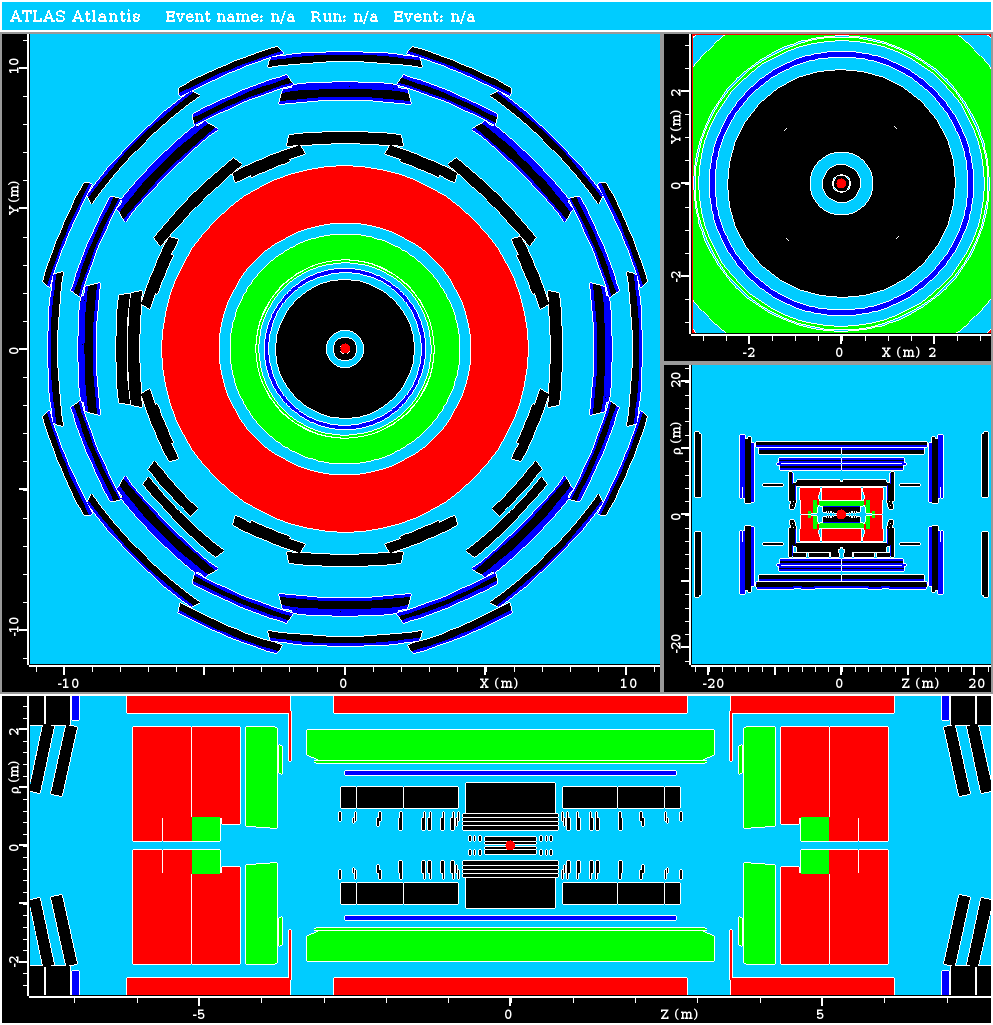
\includegraphics[width=0.8\textwidth]{./data/atlantis/atlantis_empty.png}
	\caption{Hauptfenster des Atlantis-Programms in der Standardansicht}
	\label{fig:atlantis}
\end{figure}

\section{Versuchsaufgabe 1: Darstellung von Teilchenreaktionen}

\subsection{Lerndatensätze}

Zu Beginn des Versuchs wurde der Umgang mit Atlantis geübt.
Hierzu wurden verschiedene Lerndatensätze betrachtet, die Ereignisse von Elektronen, Myonen, Photonen, $\tau$~-Leptonen und Jets enthalten.
Exemplarisch sollen für diese Teilchen im Folgenden einige Ereignisse vorgestellt werden, mit denen die Antwort des Detektors auf verschiedene Teilchenarten verstanden werden kann.

\clearpage
\subsubsection{Elektronen}
\begin{figure}[htbp]
	\centering
	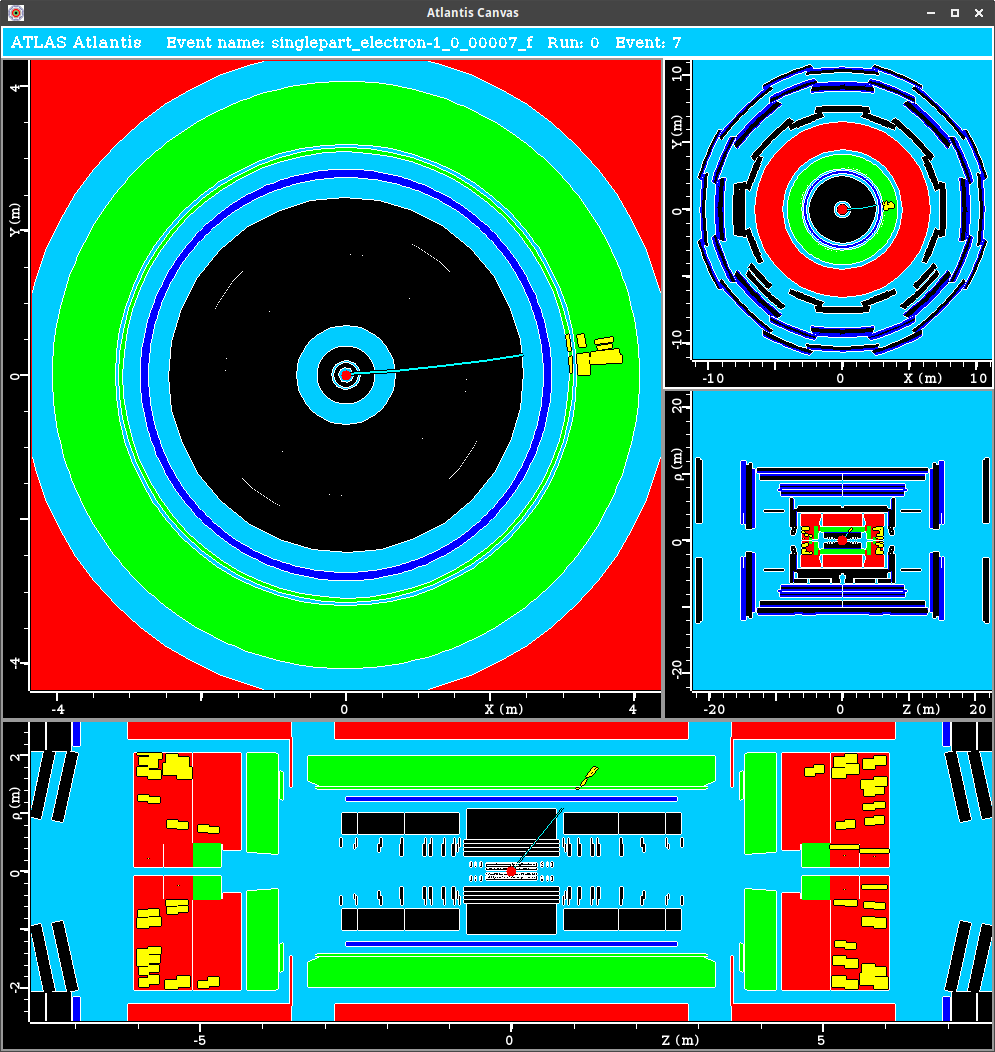
\includegraphics[width=1.0\textwidth]{./data/atlantis/singlepart_events_new/electron/curvature.png}
	\caption{Signatur eines einzelnen Elektrons im ATLAS-Detektor}
	\label{fig:electron-curvature}
\end{figure}
\vfill
\noindent
Im Lerndatensatz der Elektronen finden sich Ereignisse in denen einzelne Elektronen erzeugt wurden.
In Abbildung \ref{fig:electron-curvature} wurde ein typisches Ereignis mit einem einzelnen Elektron aufgetragen.
Die Signatur eines Elektrons ist gekennzeichnet durch eine Trajektorie im inneren Detektor, welche aufgrund der elektromagnetischen Interaktion des Elektrons mit dem Detektormaterial als Ladungseintrag in den Halbleiter- und Übergangsstrahlungsdetektoren rekonstruiert werden kann.
Das Magnetfeld im inneren Detektor, welches in Richtung der Strahlröhre zeigt, zwingt die Elektronen dort auf einen Kreisbogen und wird zur Rekonstruktion von Ladung und transversalem Impuls genutzt.
Im Fall von Abbildung \ref{fig:electron-curvature} kann an der Krümmung abgelesen werden, dass es sich um ein negativ geladenes Elektron handelt (das Magnetfeld zeigt in der $xy$-Ansicht aus der Bildebene).
Schließlich bildet das Elektron im elektromagnetischen Kalorimeter eine Kaskade aus Photonen und Elektron-Positron-Paaren aufgrund von Bremsstrahlungs- und Paarbildungsprozessen.
\vfill

\clearpage
\begin{figure}[htbp]
	\centering
	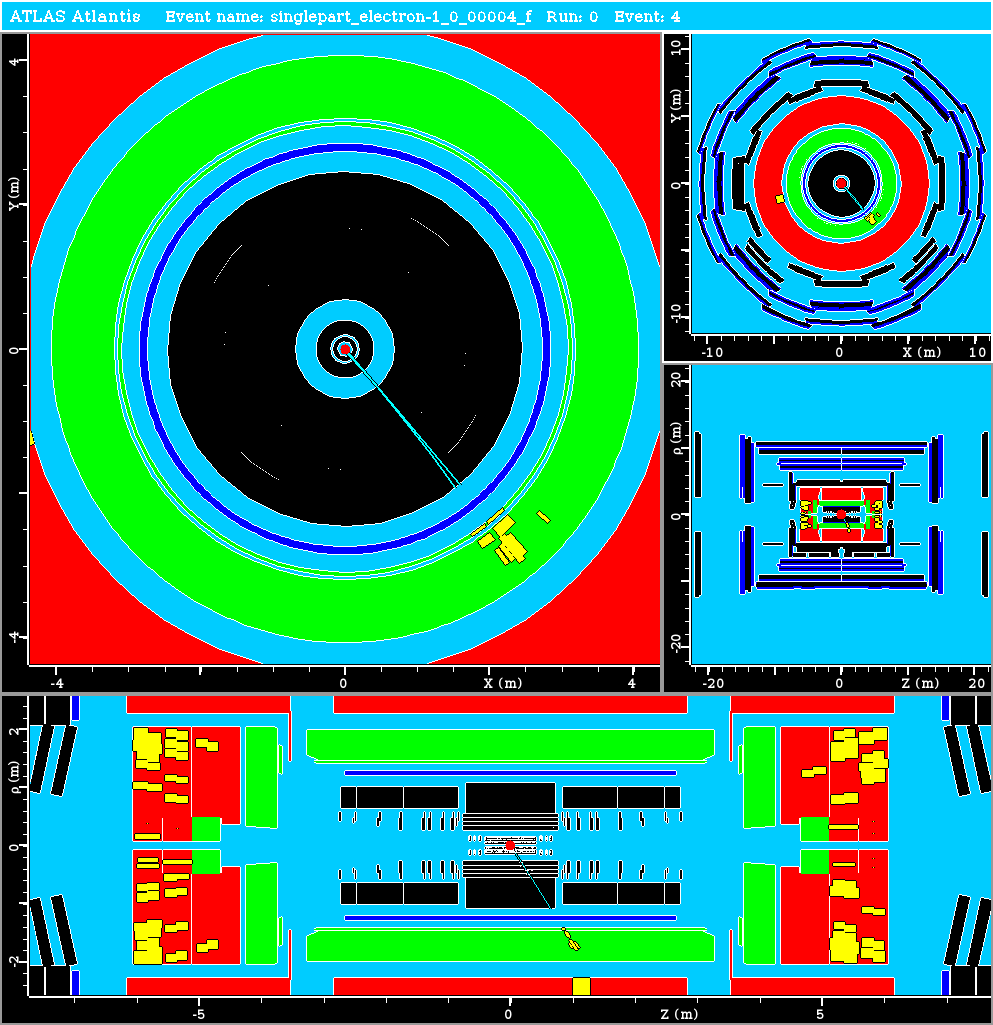
\includegraphics[width=1.0\textwidth]{./data/atlantis/singlepart_events_new/electron/twopart.png}
	\caption{Signatur eines Elektrons mit zusätzlichen geladenen Spuren im ATLAS-Detektor}
	\label{fig:electron-twopart}
\end{figure}
\vfill
\noindent
In Abbildung \ref{fig:electron-twopart} wurden zwei geladene Spuren im inneren Detektor rekonstruiert.
Da die zugrundeliegenden Ereignisse jedoch nur aus einem einzelnen Elektron bestehen, muss die zweite Spur durch das Ereignis-Elektron im Detektormaterial erzeugt worden sein.
Eine Möglichkeit dafür ist die Erzeugung eines hoch-energetischen Delta-Elektrons durch das Primärelektron.
Die Wahrscheinlichkeit für die Emission eines Delta-Elektrons in Vorwärtsrichtung ist jedoch sehr klein, daher könnte eine Alternative die Erzeugung eines Bremsstrahlphotons und die folgliche Paarbildung sein, in der das dritte Elektron nicht im Detektor rekonstruiert werden konnte.
\vfill

\clearpage
\subsubsection{Myonen}
\begin{figure}[htbp]
	\centering
	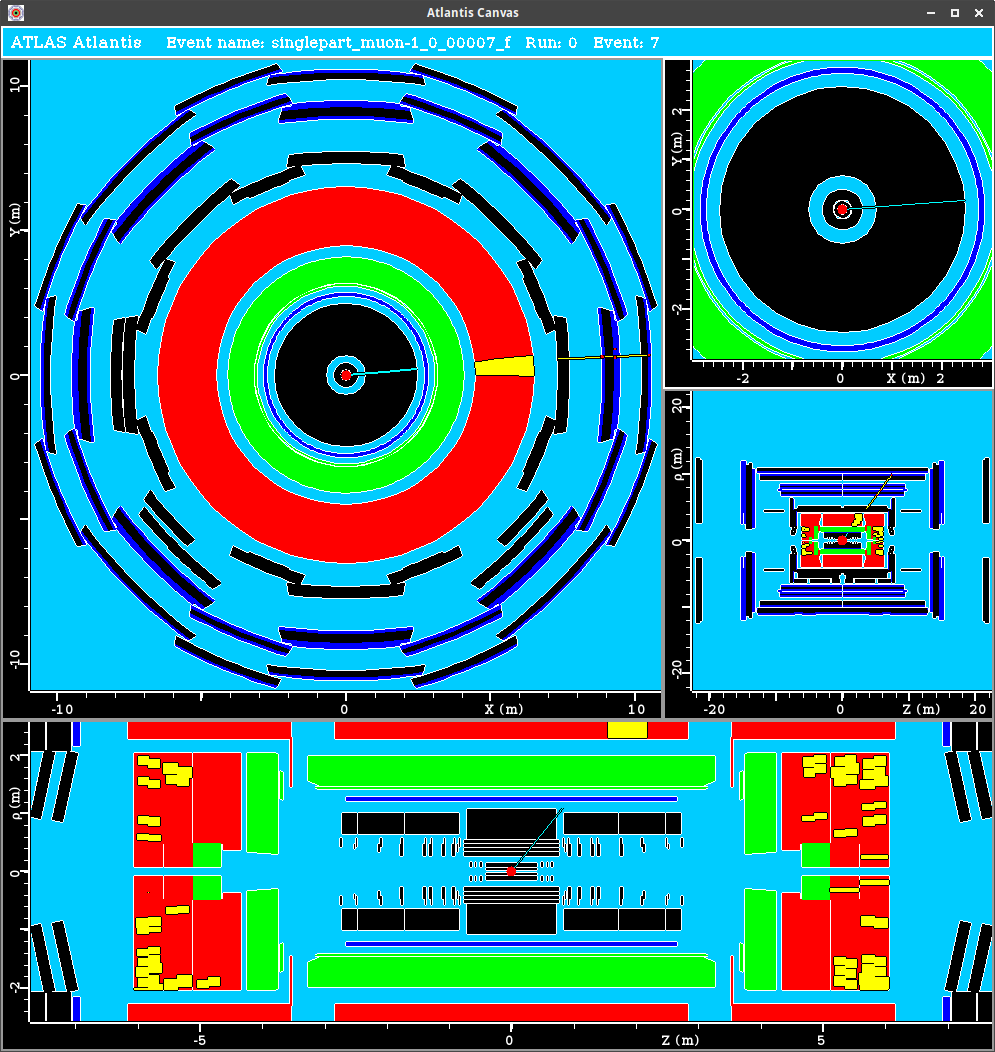
\includegraphics[width=1.0\textwidth]{./data/atlantis/singlepart_events_new/muon/single_track2.png}
	\caption{Signatur eines einzelnen Myons im ATLAS-Detektor}
	\label{fig:myon-singletrack}
\end{figure}
\vfill
\noindent
In Abbildung \ref{fig:myon-singletrack} ist die typische Detektorantwort auf ein Myon zu sehen.
Da es sich bei Myonen um geladene Teilchen handelt, hinterlassen diese eine Spur im inneren Detektor und passieren das dort anliegende Magnetfeld auf einer gekrümmten Bahn in der $xy$-Ebene.
Sie durchtreten die beiden Kalorimeter beinahe ungehindert und deponieren dabei nur eine geringe Energiemenge.
Im Myonsystem, das mit zahlreichen Detektorkammern und dem Magnetfeld eines toroidalen Spulensystems ausgestattet ist, können ebenfalls Spuren rekonstruiert werden.
Aufgrund des Magnetfeldes werden Myonen jedoch in der $\rho z$-Ebene gekrümmt, was eine zweite unabhängige Impulsmessung ermöglicht.
Da andere hadronische oder leptonische Teilchen im elektromagnetischen oder hadronischen Kalorimeter gestoppt werden und Neutrinos keine Spuren in den Detektorkammern des Myonsystems hinterlassen, ist diese Teilchensignatur auf ein Myon zurückzuführen. 
\vfill

\clearpage
\subsubsection{Photonen}
\begin{figure}[htbp]
	\centering
	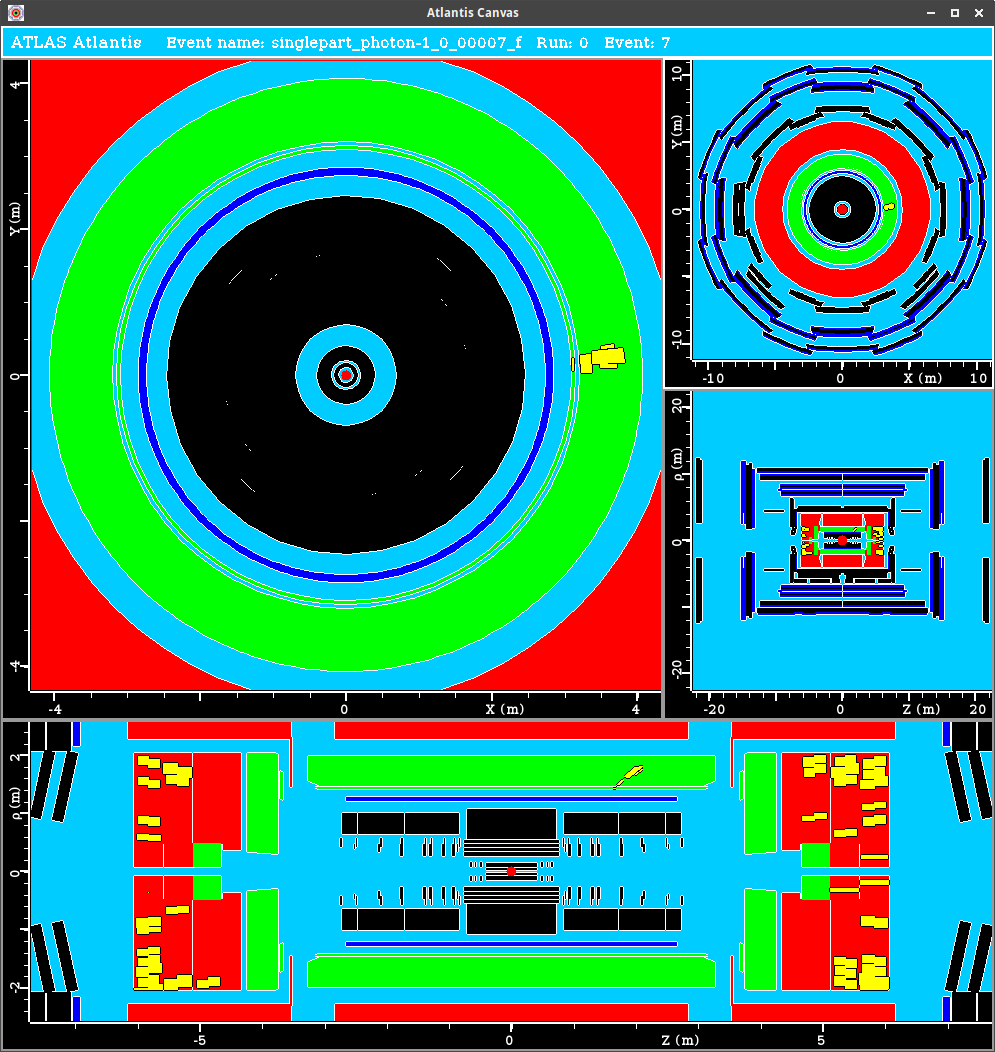
\includegraphics[width=1.0\textwidth]{./data/atlantis/singlepart_events_new/photons/single_photon_2.png}
	\caption{Signatur eines einzelnen Photons im ATLAS-Detektor}
	\label{fig:photon}
\end{figure}
\vfill
\noindent
Wie in Abbildung \ref{fig:photon} zu sehen, hinterlassen Photonen als ungeladene Teilchen keine rekonstruierbaren Spuren im inneren Detektor.
Da sie jedoch elektromagnetisch mit Materie interagieren können, formt sich im elektromagnetischen Kalorimeter ein Schauer aus Photonen und Elektron-Positron-Paaren (ähnlich zum Elektron).
In dieser Kaskade wird die gesamte Energie des Photons deponiert.
\vfill

\clearpage
\begin{figure}[htbp]
	\centering
	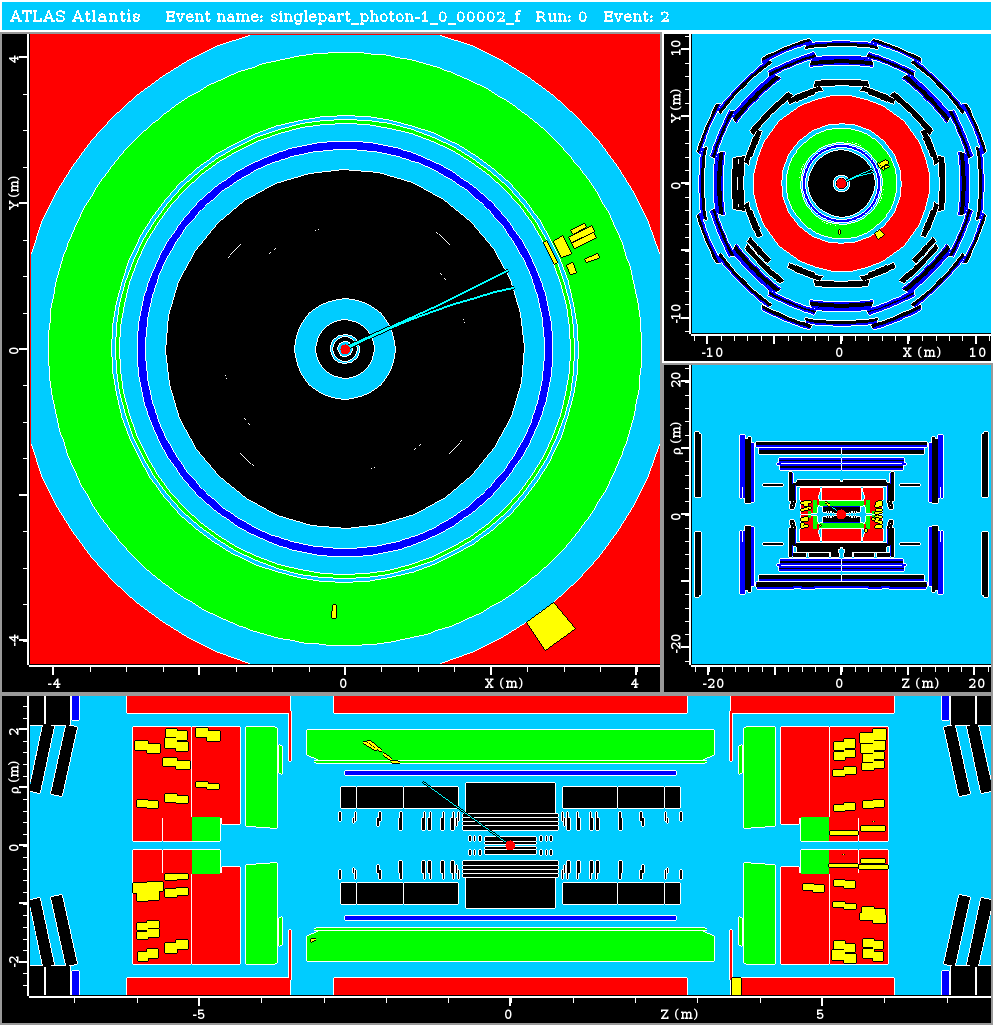
\includegraphics[width=1.0\textwidth]{./data/atlantis/singlepart_events_new/photons/conversion.png}
	\caption{Signatur eines $\ell^- \ell^+$-Paares aus dem Paarbildungsprozess eines einzelnen Photons im ATLAS-Detektor}
	\label{fig:photon-conversion}
\end{figure}
\vfill
\noindent
Im Ereignis in Abbildung \ref{fig:photon-conversion} entsteht ein Elektron-Positron-Paar durch Paarbildung des primären Photons im Detektormaterial.
Die Elektronen haben dabei entgegengesetzte Ladungen, sodass die Trajektorien im inneren Detektor in unterschiedliche Richtungen gekrümmt sind.
Darüber hinaus ist es möglich den gemeinsamen Vertex der Elektronen vom Interaktionsvertex zu unterscheiden.
Dies wurde in Abbildung \ref{fig:photon-vertex} mit der Vertexrekonstruktion von ATLANTIS dargestellt, sodass der sekundäre Vertex einen Abstand von etwa \SI{5}{\centi\meter} vom Interaktionsvertex hat.
\vfill
\begin{figure}[htbp]
	\centering
	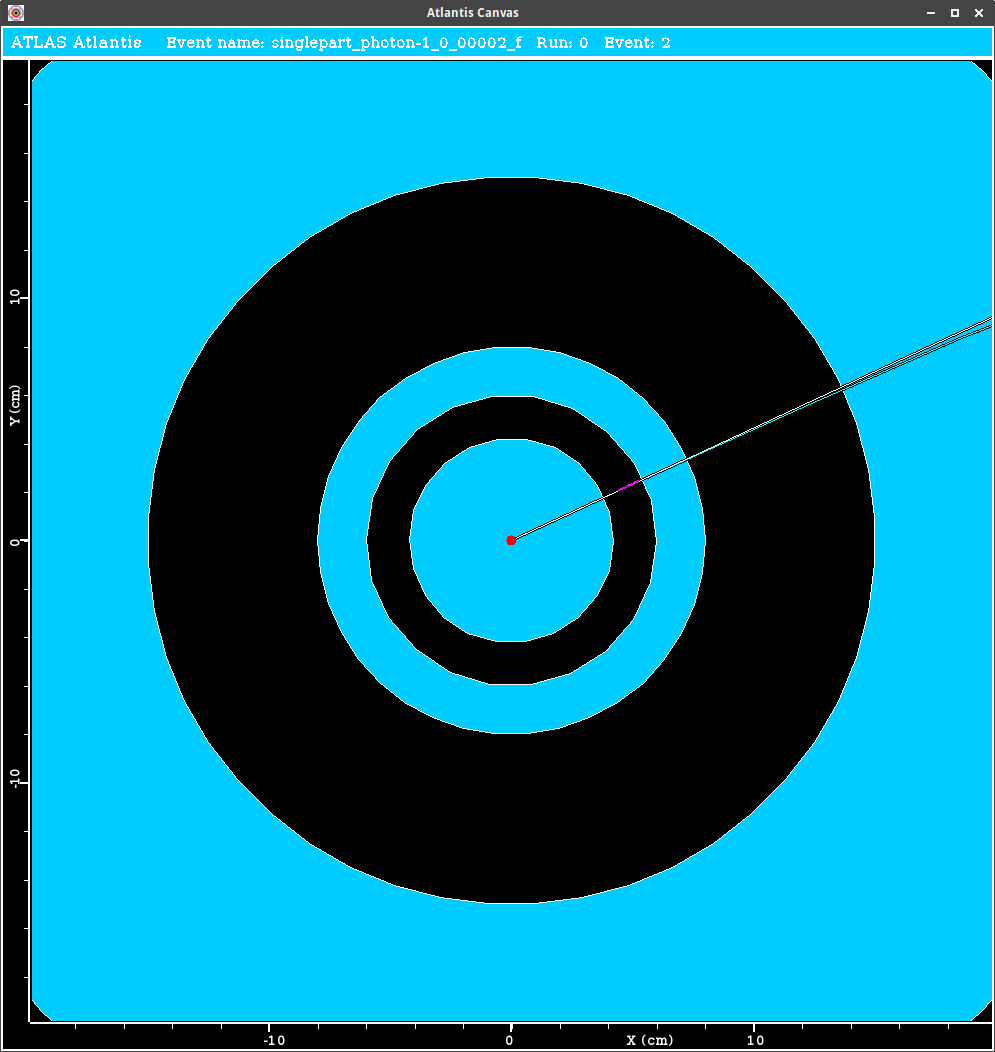
\includegraphics[width=1.0\textwidth]{./data/atlantis/singlepart_events_new/photons/conversion_vertex_no_fisheye.png}
	\caption{Von ATLANTIS rekonstruierter Vertex (magenta) des Elektron-Positron-Paars in einer Entfernung von etwa \SI{5}{\centi\meter} vom Interaktionsvertex (rot).}
	\label{fig:photon-vertex}
\end{figure}

\clearpage
\subsubsection{$\tau$-Leptonen}
\begin{figure}[htbp]
	\centering
	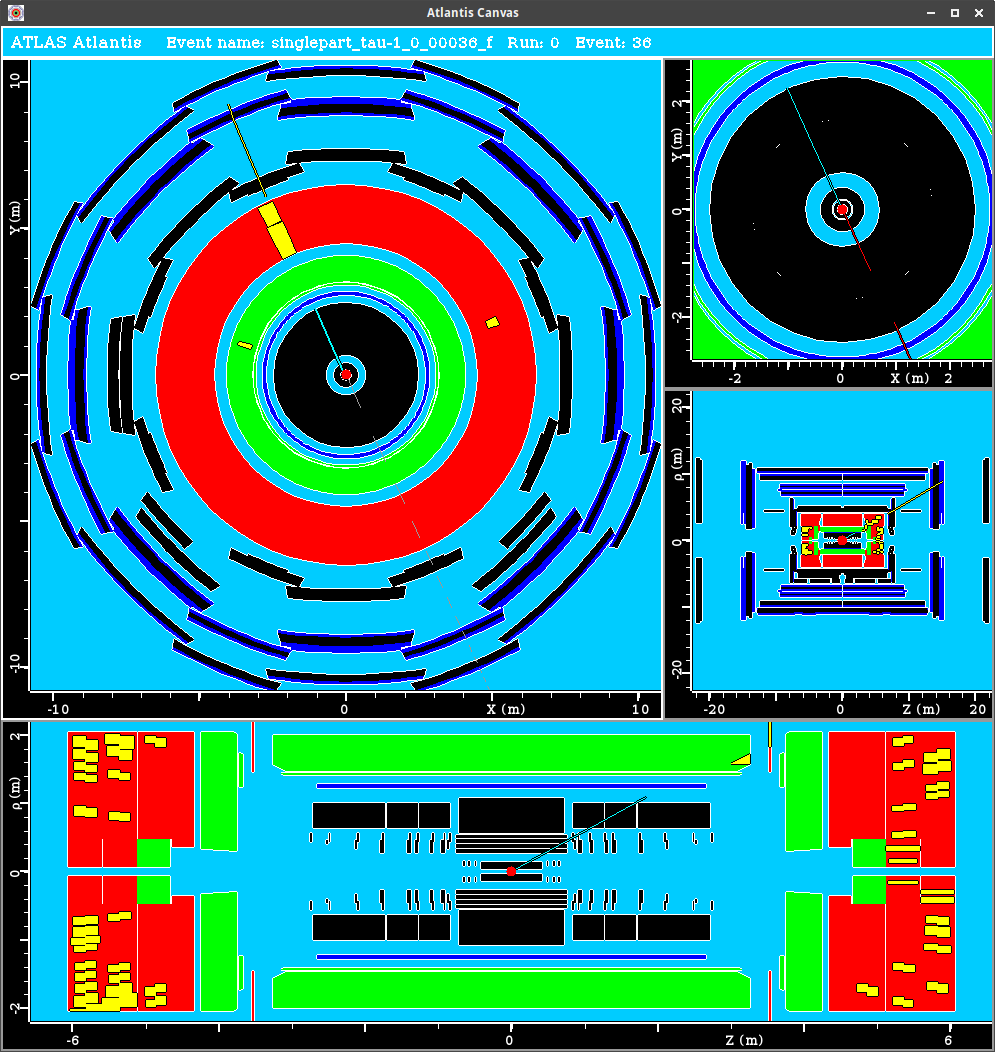
\includegraphics[width=1.0\textwidth]{./data/atlantis/singlepart_events_new/tau/muon.png}
	\caption{Signatur des leptonischen Zerfalls eines $\tau^+$-Leptons im ATLAS-Detektor.}
	\label{fig:tau-muon}
\end{figure}
\vfill
\noindent
Das Ereignis in Abbildung \ref{fig:tau-muon} des $\tau$-Lerndatensatzes zeigt den Zerfall
\begin{align*}
	\tau^+ \rightarrow \mu^+ + \nu_\mu + \bar{\nu}_\tau \, \text{.}
\end{align*}
Aufgrund der kurzen Lebensdauer zerfällt das $\tau$-Lepton nach sehr kurzer Flugstrecke $c \tau = \SI{87}{\micro\meter}$ \cite{pdg}, weshalb lediglich das Myon im Detektor rekonstruiert werden kann.
Aufgrund der Leptonen-Universalität ist auch ein Zerfall in Elektron und zugehöriges Neutrino  mit ungefähr dem gleichen Verzweigungsverhältnis (abgesehen vom Phasenraumunterschied) möglich.
Ein solcher Zerfall würde lediglich eine geladene Spur und einen Schauer im elektromagnetischen Kalorimeter verursachen und nicht wie bei dem hier betrachteten Ereignis im Myonsystem registriert werden.

In beiden Fällen entstehen zusätzlich zu dem geladenen Lepton auch ein $\tau$-Neutrino und das jeweilige Neutrino des Elektrons bzw.\ Myons.
Diese können nicht detektiert werden, die fehlende transversale Energie (in den beiden oberen Ansichten der Abbildung \ref{fig:tau-muon} rot bzw.\ grau gestrichelt) ist jedoch ein Indiz für ihre Existenz.
\vfill

\clearpage
\begin{figure}[htbp]
	\centering
	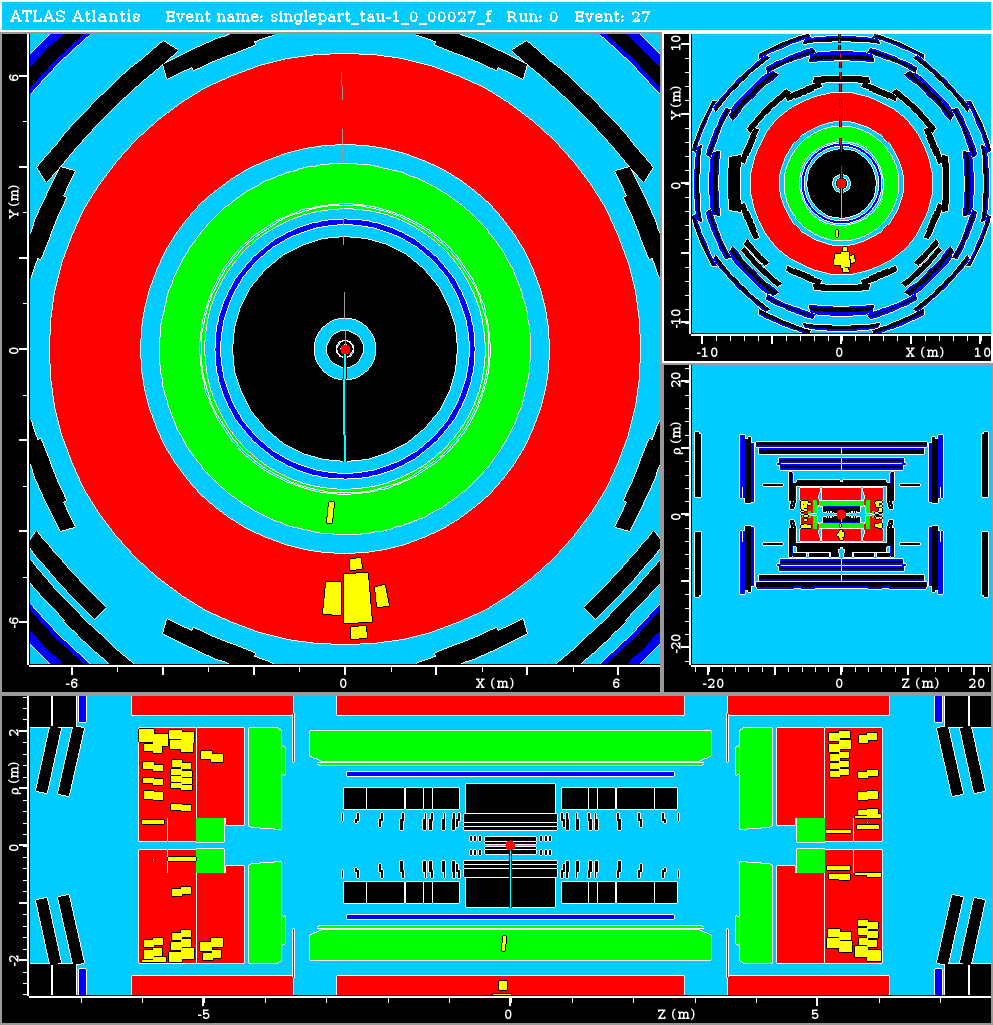
\includegraphics[width=1.0\textwidth]{./data/atlantis/singlepart_events_new/tau/single_pion.png}
	\caption{Signatur eines hadronischen $\tau$-Zerfalls im ATLAS-Detektor}
	\label{fig:tau-pion}
\end{figure}
\vfill
\noindent
Ein Beispiel für einen hadronischen $\tau$-Zerfall liefert Abbildung \ref{fig:tau-pion}.
In diesem Fall ist eine geladene Spur im inneren Detektor sichtbar, sodass ein Zerfall mit einem geladenen Pion und einem $\tau$-Neutrino im Endzustand stattgefunden haben muss.
Weiterhin können noch bis zu drei neutrale Pionen auftreten, welche nicht im inneren Detektor sichtbar sind.
Aufgrund der Lokalisierung der Energie im hadronischen Kalorimeter in einem kleinen Raumbereich ist ein Zerfall in ein einzelnes geladenes Pion zu vermuten.
Es ist ebenfalls die fehlende transversale Energie aufgrund des $\tau$-Neutrinos zu beobachten, welche im Gegensatz zum leptonischen Zerfall nun ein Maß für den transversalen Impuls des Neutrinos darstellt, da nur ein Neutrino bei diesem Ereignis auftritt.
\vfill

\clearpage
\subsubsection{Zwei-Jet}
\begin{figure}[htbp]
	\centering
	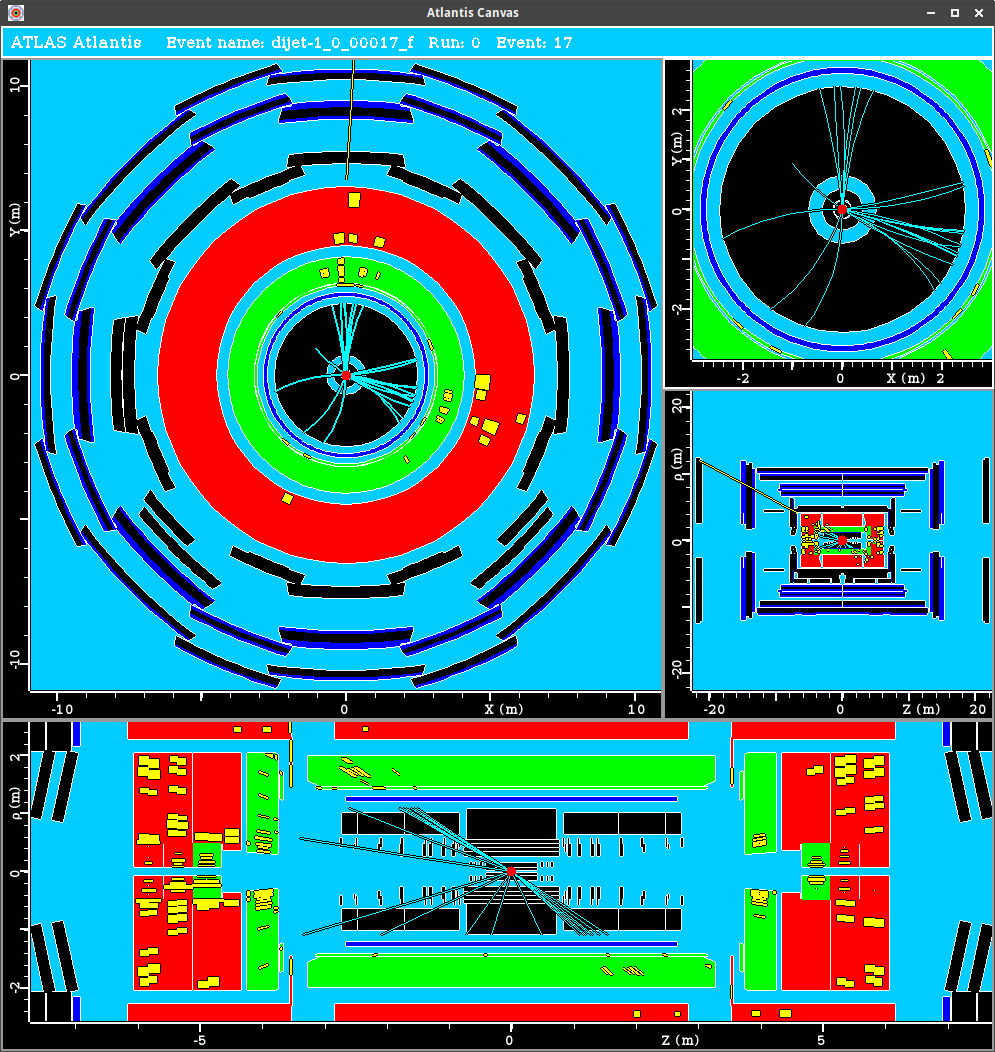
\includegraphics[width=1.0\textwidth]{./data/atlantis/singlepart_events_new/jets/muon.png}
	\caption{Signatur eines Zwei-Jet Ereignisses im ATLAS-Detektor}
	\label{fig:jets-muon}
\end{figure}
\vfill
\noindent
In dem in Abbildung \ref{fig:jets-muon} zugrundeliegenden Ereignis entstehen zwei Quarks oder Gluonen, welche folglich aufgrund des \textit{Confinements} zwischen farb-geladenen Teilchen in Mesonen und Baryonen hadronisieren.
Die so entstehenden geladenen Hadronen bilden im inneren Detektor eine Ansammlung vieler Spuren in einem engen Konus.
Ein solcher \textit{Jet} enthält sowohl geladene als auch ungeladene Pionen.
Die geladenen Pionen haben eine Zerfallslänge in der Ordnung von $c \tau = \SI{7.8}{\meter}$~\cite{pdg} und können dadurch direkt in den hadronischen Kalorimetern beobachtet werden.
Im Gegensatz dazu zerfallen die ungeladenen Pionen schnell in zwei Photonen ($c \tau = \SI{25.5}{\nano\meter}$~\cite{pdg}) und führen somit ebenfalls zu signifikanten Einträgen in den elektromagnetischen Kalorimetern.

Das Myon, welches im oberen Jet in Abbildung \ref{fig:jets-muon} zu erkennen ist, ist ein Indikator dafür, dass das hadronisierende Quark-Paar ein $b\bar{b}$-Paar gewesen ist, da der Zerfall des im Jet entstandenen B-Mesons zu einem geladenen Lepton im Endzustand führen kann.
\vfill

\subsection{Aufgabe 3: Energieverlust von Myonen im Kalorimeter}
Im Folgenden soll anhand der ersten 20 Myonen-Ereignisse aus den Lerndatensätzen der mittlere Energieverlust der Myonen in den Kalorimetern bestimmt werden. 

\subsubsection{Messung des Myonenimpulses mit Atlantis}
\label{sssec:myon_momenta}
Der ATLAS-Detektor besitzt mit dem Magnetfeld des Solenoids im inneren Detektor und dem des toroidalen Spulensystems im Myonensystem zwei unabhängige Methoden um den Myonenimpuls zu bestimmen.
Bei den betrachteten Ereignissen kann mithilfe der Ereignisanzeige \textit{Atlantis} die Myonenparameter (Impuls~$p$, transversaler Impuls~$p_\mathrm{T}$, Pseudorapidität~$\eta$, \dots) der Myonen jeweils im inneren Detektor und im Myonensystem abgefragt werden.

Um den Energieverlust der Myonen im Kalorimeter zu bestimmen, ist es nötig den Impuls~$p$ ebendieser zu bestimmen.
Da \textit{Atlantis} auf diesen Parameter jedoch keinen Fehler angibt, wurde stattdessen der transversale Impuls~$p_\mathrm{T}$ und die Pseudorapidität~$\eta$ bestimmt, um die Fehlerfortpflanzung per Hand durchzuführen.
Nach der Definition in Gleichung \eqref{eq:pseudorapidity} kann der Impuls gemäß
\begin{align*}
	p = p_\mathrm{T} \cosh(\eta)
\end{align*}
berechnet werden. \korr{evtl.\ herleiten}
Da der relative Fehler der Pseudorapidität gemäß \textit{Atlantis} in der Größenordnung $10^{-3}$ liegt, soll dieser im Folgenden vernachlässigt werden.
Dann folgt aus \textsc{Gauß}scher Fehlerfortpflanzung für den Fehler des Impulses
\begin{align*}
	\sigma_p = | \cosh(\eta) \cdot \sigma_{p_\mathrm{T}} | \, \text{.}
\end{align*}
Die Messdaten sowie die Berechnung des Impulses wurde in Tabelle \ref{tab:muon_momenta} zusammengetragen.

\begin{sidewaystable}
	\centering
	\begin{tabular}{rSSSSSSSSSS}
\toprule
{Ereignis} & {$p_T$ / \si{\GeV}} & {$\sigma_{p_T}$ / \si{\GeV}} & {$\eta$} & {$p$ / \si{\GeV}} & {$\sigma_p$ / \si{\GeV}} & {$p_T^\prime$ / \si{\GeV}} & {$\sigma_{p_T^\prime}$ / \si{\GeV}} & {$\eta^\prime$} & {$p^\prime$ / \si{\GeV}} & {$\sigma_{p^\prime}$ / \si{\GeV}} \\
\midrule
         1 &               -38.4 &                          1.0 &     1.44 &             -85.3 &                      2.3 &                      -24.1 &                                 2.6 &            1.45 &                    -53.9 &                               5.8 \\
         2 &                33.2 &                          0.8 &    -0.77 &              43.4 &                      1.0 &                       33.4 &                                 1.7 &           -0.77 &                     43.8 &                               2.2 \\
         3 &               -41.9 &                          3.6 &    -2.44 &            -241.4 &                     21.0 &                      -41.0 &                                 0.7 &           -2.44 &                   -236.9 &                               3.8 \\
         4 &                42.0 &                          0.8 &     0.57 &              48.9 &                      1.0 &                       38.1 &                                 1.3 &            0.58 &                     44.8 &                               1.6 \\
         5 &               -53.7 &                          2.1 &    -1.81 &            -168.2 &                      6.4 &                      -61.2 &                                 4.4 &           -1.73 &                   -177.6 &                              12.8 \\
         6 &                44.6 &                          1.4 &     1.62 &             117.3 &                      3.6 &                       36.6 &                                 3.1 &            1.62 &                     96.5 &                               8.3 \\
         7 &               -57.3 &                          1.7 &     0.70 &             -71.9 &                      2.1 &                      -51.8 &                                 1.1 &            0.70 &                    -65.0 &                               1.3 \\
         8 &                64.5 &                          2.7 &     1.80 &             200.0 &                      8.3 &                       64.9 &                                 2.8 &            1.79 &                    199.3 &                               8.7 \\
         9 &               -55.5 &                          1.1 &    -0.29 &             -57.8 &                      1.2 &                      -48.0 &                                 0.9 &           -0.27 &                    -49.7 &                               1.0 \\
        10 &                39.9 &                          1.0 &     1.18 &              71.1 &                      1.7 &                            &                                     &                 &                          &                                   \\
        11 &               -37.8 &                          1.2 &    -1.64 &            -100.7 &                      3.2 &                      -35.1 &                                 0.7 &           -1.65 &                    -94.3 &                               1.8 \\
        12 &                37.6 &                          0.7 &     0.19 &              38.3 &                      0.7 &                       33.9 &                                 1.2 &            0.19 &                     34.5 &                               1.2 \\
        13 &               -59.9 &                          1.8 &     1.16 &            -105.2 &                      3.1 &                      -62.1 &                                 4.2 &            1.16 &                   -108.7 &                               7.3 \\
        14 &                47.5 &                          3.3 &     2.29 &             236.1 &                     16.5 &                       53.0 &                                 1.2 &            2.29 &                    263.5 &                               5.9 \\
        15 &               -43.9 &                          1.5 &    -1.76 &            -131.7 &                      4.4 &                      -42.0 &                                 2.1 &           -1.76 &                   -125.5 &                               6.3 \\
        16 &                45.7 &                          1.8 &    -1.87 &             152.2 &                      6.1 &                       47.3 &                                 2.2 &           -1.88 &                    157.7 &                               7.2 \\
        17 &               -32.6 &                          0.5 &     0.40 &             -35.2 &                      0.6 &                      -29.8 &                                 0.5 &            0.40 &                    -32.2 &                               0.6 \\
        18 &                52.8 &                          1.1 &     0.23 &              54.2 &                      1.1 &                       48.7 &                                 2.3 &            0.23 &                     50.0 &                               2.3 \\
        19 &               -64.5 &                          2.5 &     0.77 &             -84.7 &                      3.3 &                      -52.2 &                                 1.0 &            0.76 &                    -68.1 &                               1.4 \\
        20 &                47.6 &                          1.3 &     1.42 &             104.2 &                      2.9 &                       49.5 &                                 3.2 &            1.42 &                    108.0 &                               7.0 \\
        21 &               -35.5 &                          2.3 &    -2.33 &            -184.1 &                     11.8 &                      -33.2 &                                 0.8 &           -2.32 &                   -170.8 &                               4.0 \\
\bottomrule
\end{tabular}

	\caption{Bestimmung des Impulses des Myons im inneren Detektor (ungestrichene Größen) und im Myonensystem (gestrichene Größen) mithilfe der gemessenen Pseudorapidität~$\eta$ und des transversalen Impulses~$p_\mathrm{T}$.
		Für Ereignis 10 konnte kein äußeres Myon rekonstruiert werden (für weitere Erklärung siehe Abschnitt \ref{sssec:myon_momenta}) stattdessen wurde noch das 21.\ Ereignis in die Analyse einbezogen.}
	\label{tab:muon_momenta}
\end{sidewaystable}

\subsubsection{Bestimmung von Impuls- und Energieverlust der Myonen im Kalorimeter}

\begin{align*}
	\Delta p = p - p^\prime
\end{align*}
Hier ergibt sich der quadratische Fehler aus quadratischer Addition der Fehler.

\begin{align*}
	E &= \sqrt{m_\mu^2 + p^2} \\
	\sigma_E &= \sqrt{\frac{p^2 \, \sigma_p^2}{m_\mu^2 + p^2}}
\end{align*}

\begin{align*}
	m_\mu \approx \SI{105.658}{\MeV} \, \cite{pdg}
\end{align*}


\begin{sidewaystable}[h]
	\centering
	\begin{tabular}{rSSSS}
\toprule
{Event} & {$p_T$ / \si{\GeV}} & {$\Delta p_T$ / \si{\GeV}} & {$E_\mathrm{loss}$ / \si{\GeV}} & {$\Delta E_\mathrm{loss}$ / \si{\GeV}} \\
\midrule
      1 &               -38.4 &                        1.0 &                            31.4 &                                    6.2 \\
      2 &                33.2 &                        0.8 &                            -0.4 &                                    2.4 \\
      3 &               -41.9 &                        3.6 &                             4.5 &                                   21.3 \\
      4 &                42.0 &                        0.8 &                             4.1 &                                    1.8 \\
      5 &               -53.7 &                        2.1 &                            -9.4 &                                   14.3 \\
      6 &                44.6 &                        1.4 &                            20.8 &                                    9.1 \\
      7 &               -57.3 &                        1.7 &                             7.0 &                                    2.5 \\
      8 &                64.5 &                        2.7 &                             0.7 &                                   12.1 \\
      9 &               -55.5 &                        1.1 &                             8.1 &                                    1.5 \\
     10 &                39.9 &                        1.0 &                                 &                                        \\
     11 &               -37.8 &                        1.2 &                             6.4 &                                    3.6 \\
     12 &                37.6 &                        0.7 &                             3.8 &                                    1.4 \\
     13 &               -59.9 &                        1.8 &                            -3.5 &                                    8.0 \\
     14 &                47.5 &                        3.3 &                           -27.4 &                                   17.5 \\
     15 &               -43.9 &                        1.5 &                             6.2 &                                    7.7 \\
     16 &                45.7 &                        1.8 &                            -5.5 &                                    9.5 \\
     17 &               -32.6 &                        0.5 &                             3.1 &                                    0.8 \\
     18 &                52.8 &                        1.1 &                             4.2 &                                    2.6 \\
     19 &               -64.5 &                        2.5 &                            16.7 &                                    3.6 \\
     20 &                47.6 &                        1.3 &                            -3.8 &                                    7.6 \\
     21 &               -35.5 &                        2.3 &                            13.3 &                                   12.5 \\
\bottomrule
\end{tabular}

	\caption{Testtabelle}
\end{sidewaystable}

\begin{figure}[h]
	\centering
	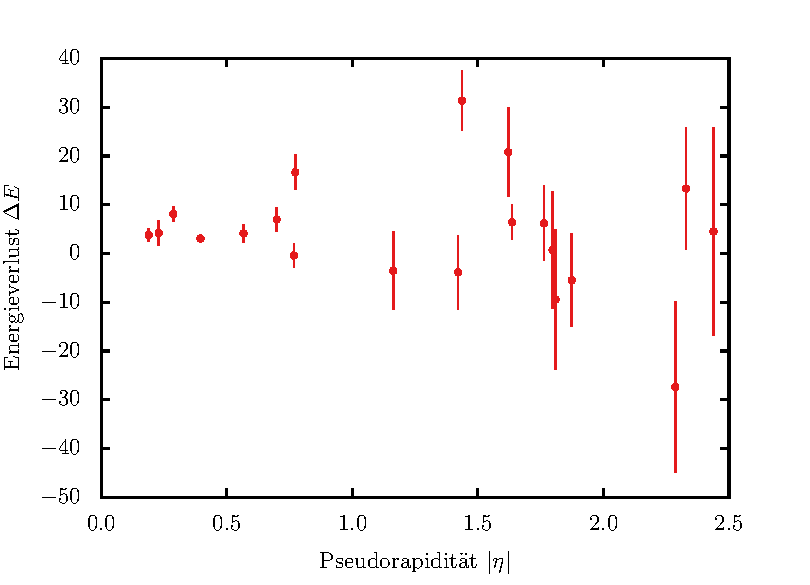
\includegraphics{./figures/muon_energy_loss/eta.pdf}
	\caption{Energieverlust von Myonen im ATLAS-Detektor}
\end{figure}

\begin{figure}[h]
	\centering
	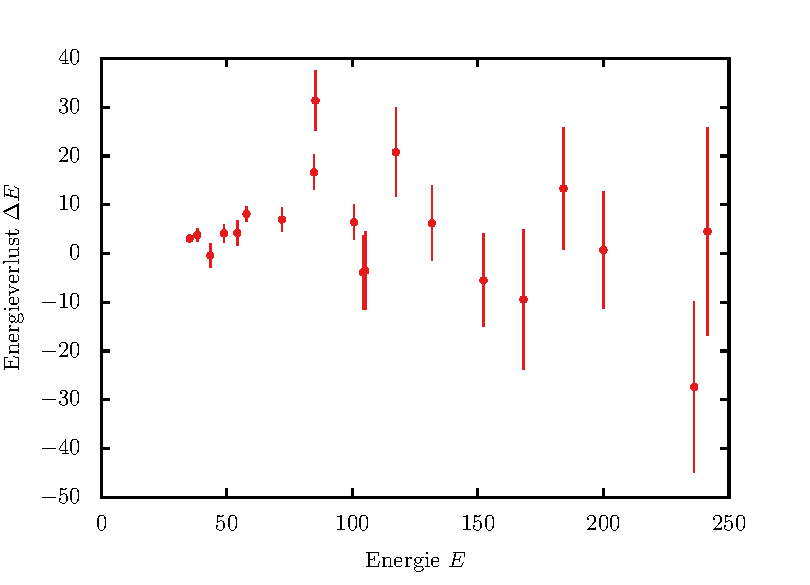
\includegraphics{./figures/muon_energy_loss/energy.pdf}
	\caption{Energieverlust von Myonen im ATLAS-Detektor}
\end{figure}

\subsection{Aufgabe 6: invariante Elektron-Positron-Masse}

\FloatBarrier
% BIBLIOGRAPHIE
\vspace{\fill}
% Maximale Anzahl der Einträge in Klammer
% Zitieren mit \cite{lamport94}
\begin{thebibliography}{19}
\bibitem{pdg}
	K.A. Olive \textit{et al.} (Particle Data Group),
	\emph{The Review of Particle Physics},
	Chin. Phys. C, \textbf{38}, 090001 (2014).
	
\bibitem{leo}
	W. R. Leo,
	\emph{Techniques for Nuclear and Particle Physics Experiments},
	Springer 1994

\end{thebibliography}

% APPENDIX
\begin{appendix}
\newpage
\section{Anhang}

\FloatBarrier
\subsection{Section in Appendix}
Appendix
\FloatBarrier

\end{appendix}

\end{document}
